\documentclass[10pt]{article}
\usepackage[utf8]{inputenc}
\usepackage[spanish]{babel}
\usepackage[usenames,dvipsnames,svgnames,table]{xcolor}
\usepackage{multirow}
\usepackage{diagbox}
\usepackage{booktabs}
\usepackage{anysize} 
\usepackage{hyperref}
\usepackage{helvet}
\renewcommand\refname{Referencias}
\marginsize{2cm}{2cm}{2.0cm}{2cm}
\usepackage{enumitem}
\usepackage{setspace}
\usepackage{scrextend}
\usepackage{amssymb}
\usepackage{mathtools}
\addtokomafont{labelinglabel}{\sffamily}

%% Graphics
\usepackage{graphicx}
\usepackage{color}
\usepackage{gensymb}
\usepackage{multirow}
\usepackage{caption}
\usepackage{float}
\graphicspath{{img/}}
\setlength{\parindent}{0cm}


\hypersetup{
	colorlinks=true,
	linkcolor=blue,
	filecolor=magenta,
	urlcolor=cyan,
	citecolor=blue
}




\begin{document}
	\title{Fundamentos de Bases de Datos \\
		Proyecto Final\\ Empresas Inmobiliarias
	} 
	\author{Díaz Gómez Silvia \\
		Eugenio Aceves Narciso Isaac \\
		Quiroz Castañeda Edgar}
	\date{08 de Junio del 2019}
	\maketitle
	
	A continuación se enlistan los archivos de este proyecto separados por carpetas:\\
	\begin{itemize}
		\item Doc : En este directorio se la documentación.
		\begin{description}[leftmargin=8em,style=nextline]
			\item[Especificacion] En este documento se explica todas las decisiones del diseño para la base de datos.
			\item [Reporte] En este documento se muestran los resultados de la evaluación de las consultas correspondientes al archivo consultas.sql.
			\item[dicc\_tablas] Archivo csv con el diccionario de datos.
			\item[dicc\_constrains] Archivo csv con la informacion de las restricciones de la base de datos.
			\item[Imagenes] Directorio que contiene todas las imagenes necesarias para la generación del reporte y la especificación. 
		
	    \end{description}	
		\item Esquema : En este directorio se encuentran archivos .Dia con los diagramas correspondientes al diseño de la base de datos. 
		\begin{description}[leftmargin=8em,style=nextline]
			\item[modeloER] Diagrama Modelo entidad-Relación de la base de datos.
			\item[modeloRelacional] Diagrama que corresponde a la traducción del diagrama del modelo Entidad-Relación.
			\item[modeloNormalizado] Contiene el diagrama relacional normalizado. 
		\end{description} 
		\item Scripts: En este directorio se encuentran los archivos SQL.
		\begin{description}[leftmargin=8em,style=nextline]
			\item[tblspace] Archivo que crea un tablespace y un usuario.
			\item[DDL] Archivo donde se crean las tablas correspondientes a la base de datos.
			\item[MOCK\_DATA] Archivo que llena la base de datos.
			\item[CONSULTAS] Archivo con algunas consultas.
			\item[STORED]  Archivo que crea los disparadores y procedimientos almacenados para la base de datos.
		\end{description}
	\end{itemize} 
	
	Se nos pide diseñar una base de datos para poder almacenar toda la información que  las inmobiliarias han proporcionado. Como el almacenamiento de la información debe estar en una base de datos relacional el diseño consta de tres partes, la primera parte corresponde al modelo Entidad-Relación, la segunda parte a la traducción del modelo entidad relación al modelo relacional y finalmente la normalización que nos permite quitar redundancia en las tablas generadas. 
	
	\section{Modelo E/R}
	
	A continuación se presenta la explicación del diseño de acuerdo al modelo entidad-relación.
	
	\subsection{Entidades} 
	\begin{itemize}
		\item Fuertes
		\begin{description}[leftmargin=8em,style=nextline]
			\item [Propiedad] Esta entidad es necesaria ya que se nos pide llevar un control sobre propiedades. Tiene como atributos 
			\textit{Id\_propiedad} es la llave primaria para esta endidad, \textit{dirección, tamaño, fecha\_construccion, valor catastral, estado propiedad, antigüedad } este ultimo es una tributo calculado.\\
			
			\item [Colonia] Se decidio crear esta entidad para saber la colonia en que se encuentra una propiedad y conocer si cerca de las propiedades se hay algun servicio de transporte público y tiendas departamentales. Tiene como atributos \textit{Nombre, CP, numero de habitantes}.\\
			
			\item [Dueño] Esta entidad sirve para llevar el control de los dueñosd e las propiedades. Tiene como atributos \textit{ id\_dueño} que corresponde a la llave primaria y \textit{monto\_invertido} que indica cuanto dinero a invertido el dueño para reparar a la propiedad adquirida.\\
			
			\item [Inmobiliaria] Esta entidad representa las empresas que adquieren las propiedad y unicamente tiene el atributo \textit{id\_inmobiliaria} que funciona como identificador unico.\\
			
			\item [Estado] La intención de esta entidad es porque es importante saber en que estados de la republica mexicana se encuentran las propiedades.  Tiene como atributo \textit{nombre}.\\
			
			
			\item [Seguro] Las propiedades pueden contar con un seguro por lo tanto se decidio crear esta entidad que administra esta información. Los atributos importantes para esta entidad son \textit{numero de poliza} que funciona como la llave primaria, \textit{monto\_anual, cobertura, empresa}.\\
			
			\item [Inmueble] Esta entidad se deriva de propiedad, casa y departamento son inmuebles y como existen cosas en comun para estas dos se vio necesario crear esta entidad, por lo tanto esta entidad funciona como entidad padre.\\
			
			\item [Casa] Es la entidad hijo de inmueble y como nos interesa cosas especificas para las propiedades que son casas se crea esta entidad.\\
			
			\item [Departamento] Al igual que casa, se necesita saber tener información de propiedades que son departamentos por lo tanto es necesario crear un entidad departamento que deriva de inmueble.\\
			
			\item [Terreno] Terreno se deriva de propiedad. Es necesaria una entidad terreno ya que representa la extensión de superficie y no necesariamente tiene una construcción y como si nos interesa saber si tiene o no alguna construcción distinta a una casa o departamento entonces tiene como atributo construcción que es de tipo boolean.
			
			\item [Edificio] Esat entidad fue necesaria crearla porque necesitamos conocer si el edificio donde se encuentra un departamentos tiene ciertas amenidades como esta infomación no se puede poner en la entidad departamento fue necesario hacer otra entidad que contuviese esa información.
			
			
		\end{description}
		\item Débiles
		\begin{description}[leftmargin=8em,style=nextline]
			\item [Municipio] Esta entidad representa a los municipios y fue necesaria crearla ya que también nos interesa conocer el municipio en donde se ubica alguna propiedad, es un entidad debil porque los nombres de municipios no son unicos así que al ser entidad debil siempre estara asociado a la infomación la entidad estado.\\
			
			\item [Transporte] Representa a un catalogo que indica una estación de metro, una base de taxis, una parada de algun otro transporte público y es una entidad debil porque debe estar asiciado a una colonia.\\
			\item [Tienda departamental] De la misma forma que la entidad transporte es necesaria una entidad tienda departamental que contiene la infomación de posibles tiendas departamentales que puedan haber en una determinda colonia.\\
		\end{description}
	\end{itemize}
	
	\subsection{Relaciones}
	\begin{itemize}
		\item Fuertes
		
		\begin{description}[leftmargin=9em,style=nextline]
			\item[Ser dueño] Esta relación esta asociada con la entidad propiedad 
			y dueño. Además esta relación tiene atributos que nos permite tener acceso a infomación especifica sobre la cantidad, la fecha de compra y la fecha en la que se dejo de ser dueño de la propiedad.\\
			
			\item[Contar] Relación que esta asociada con servicios y propiedad y es una relacion de uno a muchos ya que una propiedad puede tener muchos servicios. \\
			
			\item[Pertenecer] Relación que asocia a la entidad colonia y propiedad, es una relación de uno a muchos porque muchas propiedades pueden estar en una misma colonia. \\
			
			\item[Ubicar] Relación de uno a muchos, muchas colonias pueden estar en un mismo municipio. Une la entidad colonia con municipio.\\
			
			\item[Vender] Esta relación esta asociada con la entidad propiedad y asesor y permite conocer la infomación de la venta de una propiedad, tiene como atributos el precio que es la cantidad a la que se vendio dicha propiedad y la fecha que indica la fecha de la venta.\\
			
			\item[Situar] Relación de pertenencia y relaciona la entidad departamento con edificio.\\
			
			\item[Revender] Esta relación esta asociada con la entidad propiedad e inmobiliaria, ya que una inmobiliaria puede vender las propiedades adquiridas y es necesario llevar un control de esta por lo tanto tiene como atributos el precio y la fecha de la venta. Es una relación de uno de muchos ya que una inmobiliaria puede vender varias propiedades.\\
			
			\item[Tener] Es una relación entre propiedad y seguro, es una relación de uno a muchos porque una propiedad puede tener varios seguros.\\
			
			\item[Venta historial] Esta relación nos sirve para poder tener infomación de las variaciones en los precios de las propiedades, que será un control mensual. \\
			
			\item[Ser encargado] Relaciona la entidad propiedad y asesor, y es una relación de muchos a muchos porque muchas propiedades pueden estar a cargo de varios asesores. \\
			
		\end{description}
	\item Débiles
\begin{description}[leftmargin=8em,style=nextline]
			
			\item[Estar] Es una relación de pertenencia que asocia un estado a un municipio. Relación de uno a muchos porque un estado puede tener varios municipios.\\
			
			\item[Tener transporte] Es una relación de pertenencia que asocia algun tipo de transpote público a una colonia. Relación de uno a muchos porque una colonia puede tener asociados varios tipos de transporte públicos. \\
			
			\item[Tener tienda] Es una relación de pertenencia que asocia a tienda departamental con colonia. Relación de uno a muchos porque en una colonia pueden encontarse varias tiendas departamentales. 
		\end{description}
	\end{itemize}
	
	
	
	En la siguiente figura \ref{ER} representa lo que se ha explicado en la parte de arriba.
	
	\begin{center}
		\begin{figure}[H]
			\centering
			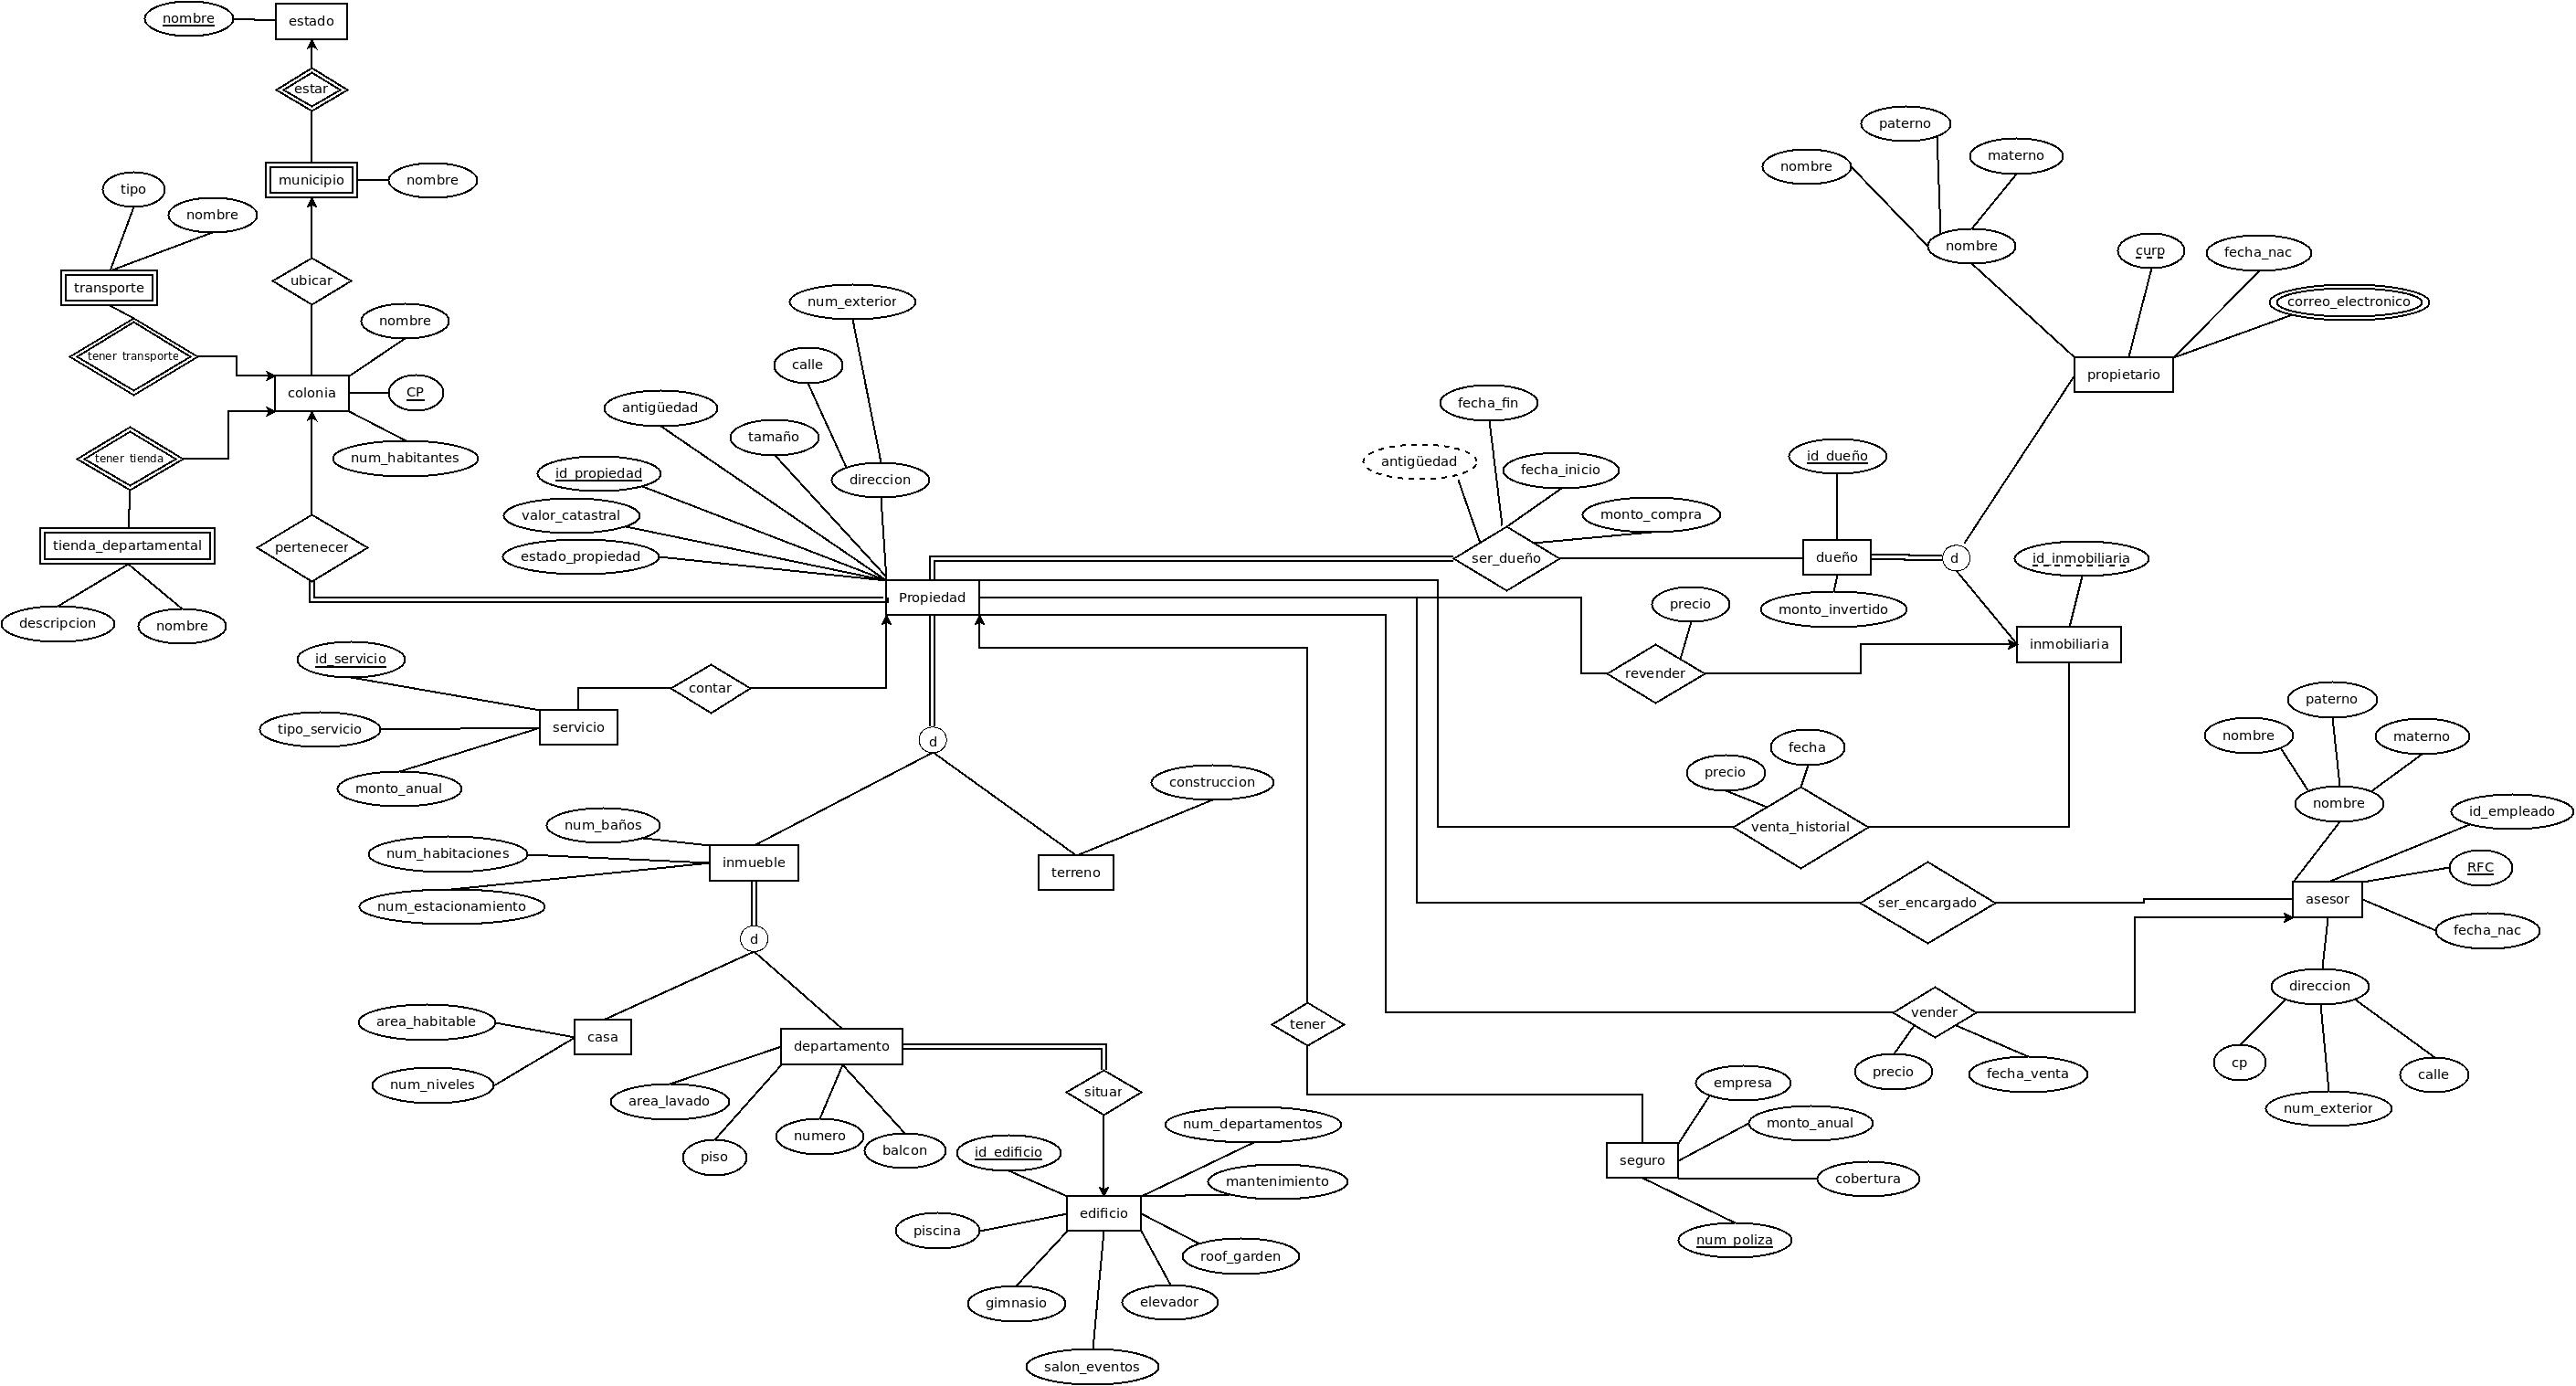
\includegraphics[width=1 \textwidth]{modeloER.jpeg}
			\caption{Diagrama E-R para las empresas inmobiliarias.}
			\label{ER}
		\end{figure}
	\end{center}
    \section{Modelo Relacional}
    
    Esta sección consiste en hacer la traducción del diagrama Entidad-Relación de la figura \ref{ER} al modelo relacional donde se debe indicar las llaves primarias para cada tabla que se genere y sus correspondientes llaves foraneas.
    
    \begin{description}[leftmargin=9em,style=nextline]
    	\item[Estado] Esta entidad se convierte en una tabla y su llave primaria es el unico atributo que tiene que es \underline{nombre}.
    	\item[Estar] Esta relación pasa como llave foránea a Municipio. 
    	\item[Municipio] Pasa a ser una tabla y tiene como llave primaria la combinación de los atributos \underline{nombre} y \underline{nombre\_estado}.
    	\item[Colonia]  Esta entidad se convierte en una tabla y tiene como llave primaria el código postal \underline{CP}. Además tiene como llaves foraneas a los identificadores de la entidad municipio.
    	\item[Transporte] Esta entidad debil se convierte en una tabla y su llave primaria esta compuesta por sus tres atributos \underline{nombre}, \underline{tipo} y \underline{CP}.
    	\item[Tener transporte] Pasa como llave foránea a la tabla Transporte.
    	\item[Tienda departamental] Esta entidad débil pasa a ser una tabla y su llave primaria se compone de los atributos \underline{nombre} y \underline{CP}.
    	\item[Tener tienda] Pasa como llave foránea a la tabla Tienda departamental.
    	\item[Propiedad] Esta entidad se convierte en tabla y su llave primaria es \underline{id\_propiedad}.
    	\item[Contar] Pasa como llave foránea a la tabla servicio.
    	\item[Servicio] Se convirte en una tabla y tiene como llave primaria \underline{id\_servicio}, además tiene como llave foránea id\_propiedad.
        \item[Ser dueño] La relación ser dueño se convierte en una tabla, teniendo como llaves foráneas id\_dueño y id\_propiedad.
   	    \item[Dueño] Pasa a ser una tabla que tiene como llave primaria \underline{id\_dueño}.
   	    \item[Revender] Esta relación se convierte en una tabla y tiene como llaves foráneas id\_propiedad, id\_dueño y id\_inmobiliaria.
   	    \item[Inmbobiliaria] Se convierte en una tabla que tiene como llave primaria id\_inmobiliaria y id\_dueño. Además tiene como llave foránea al identificador de dueño.
    	\item[Venta historial] Se convierte en un tabla que tiene como llaves foráneas a los identificadores de Propiedad e Inmobiliaria.
    	\item[Ser encargado] Pasa a ser una tabla con llaves foráneas los identificadores de Propiedad y Asesor.
    	\item[Asesor] Se convierte en una tabla que tiene como llave primara el atributo \underline{RFC}.
    	\item[Inmueble] Se convierte en un tabla que tiene como llave primaria a \underline{id\_propiedad}, y tiene como llave foránea al identificador de Propiedad.
    	\item[Terreno] Se convierte en un tabla que tiene como llave primaria a \underline{id\_propiedad}, y tiene como llave foránea al identificador de Propiedad.
    	\item[Casa] Pasa a ser una tabla donde su llave primaria es \underline{id\_propiedad}, y tiene como llave foránea al identificador de Propiedad.
    	\item[Departamento]  Pasa a ser una tabla donde su llave primaria es \underline{id\_propiedad}, y tiene como llaves foráneas a los identificadores de Propiedad y Edificio.
    	\item[Edificio] Se convierte en una tabla y su llave primaria es id\_edificio.
    	\item[Situar] Pasa como llave foránea a Departamento.
    	\item[tener] Pasa como llave foránea a Seguro.
    	\item[Seguro] Se convierte en tabla y su llave primaria es su atributo \underline{num\_poliza} y tiene como llave foránea al identificador de Propiedad.
   \end{description} 	
    
    
    En al figura \ref{MR} se muestra como queda el esquema de acuerdo a lo que se explicó anteriormente.
    \begin{center}
    	\begin{figure}[H]
    		\centering
    		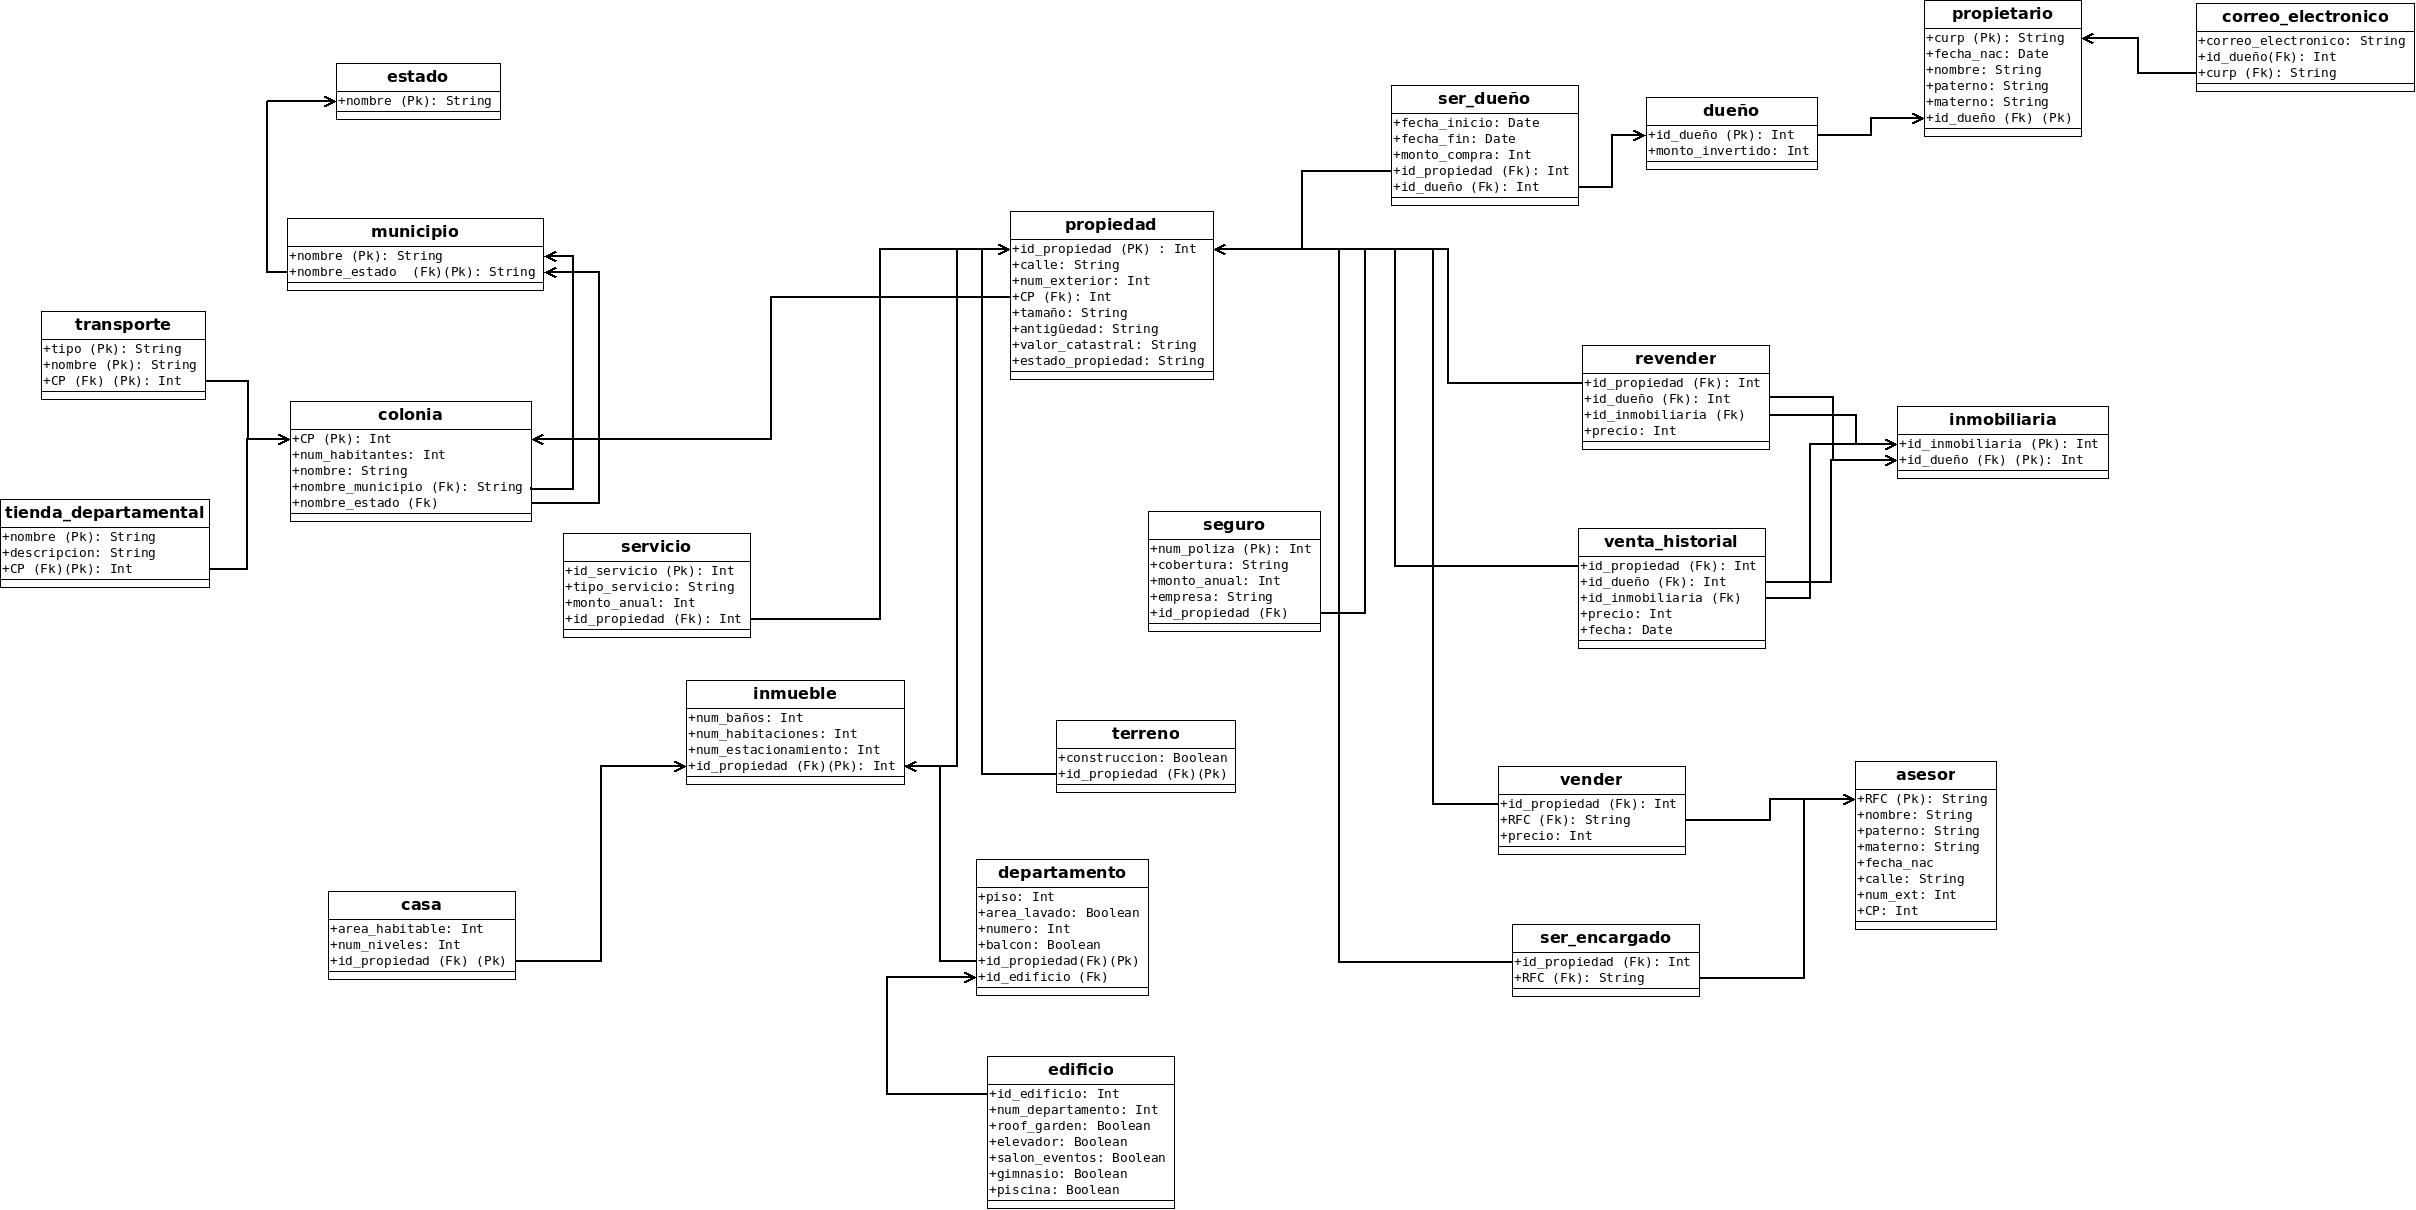
\includegraphics[width=1 \textwidth]{modeloRelacional.jpeg}
    		\caption{Traducción del diagrama del la figura \ref{ER} al modelo Relacional.}
    		\label{MR}
    	\end{figure}
    \end{center}

    \section{Normalización}
    
    Aquí se enlistan las relaciones que contenian dependencias funcionales triviales por lo tanto no fue necesario normalizarlas. 
    Todas las relaciones con únicamente dos atributos ya está normalizadas, pues las
    únicas dependencias funcionales que pueden haber son las triviales o las inducidas
    por llaves (un atributo determina al otro), y ninguna de estas es violación a la forma normal de BCNF.
    \begin{itemize}
    	\item Inmueble
    	\item Casa
    	\item Terreno
    	\item Departamento
    	\item Edificio
    	\item Ser dueño
    	\item Dueño
    	\item Correo 
    	\item Venta historial
    	\item Revender
    	\item Inmobiliaria
    	\item Vender
    	\item Ser encargado
    \end{itemize}
    
    En seguida se encuentran las relaciones que contienen dependencias no triviales o redundantes. Normalizamos de acuerdo a BCNF.
    
    \begin{enumerate}
    	\item \textbf{Colonia}
    	
    	La relación colonia es:
    	\[\overbrace{{\textbf{Colonia}}}^{\textbf{$R_{C}$}} 
    	(
    	\overbrace{CP}^{A}, \overbrace{num\_habitantes}^{B},
    	\overbrace{nombre}^{C}, \overbrace{nombre\_municipio}^{D}, \overbrace{nombre\_estado}^{E}
    	)
    	= 
    	\textbf{$R_C$}(A,B,C,D,E)
    	\]
    	
    	Y las dependencias funcionales encontratas en esta relación  y no triviales son:\\
    	\[\mathcal{F} = \{A \rightarrow CDE\}\]
    	
    	Lo siguiente sera determinar una llave para la relacion $R_C$ calculando la cerradura de la parte que se encuentran a la izquierda de las dependencias funcionales. La llave nos permitirá conocer si existen violaciones a la forma normal de BC.\\
    	
    	$\{\textcolor{RoyalBlue}{A}\}+= \{\textcolor{RoyalBlue}{A}CDE\}$\\
    	
    	El atributo $A$ casi alcanza a la mayoria de todos los atributos excepto a $B$, así que una llave para $R_C$ puede ser \textbf{AB}, ninguna de las dependecias funcionales cumple que la llave se encuentre a la izquierda de las dependencias funcionales por lo tanto son violaciones a BCNF.\\
    	\begin{itemize}
    		\item Para $A \rightarrow CDE$\\
    		Dividimos en dos relaciones la relacion original de acuerdo a los atributos de esta dependencia funcional, para la primera relación queda como:\\
    		
    		$\textbf{T}(A,C,D,E)$ con $A \rightarrow CDE$\\
    		
    		y para la suguiente relación se toman los atributos del lado izquierdo y los atributos restantes.\\
    		
    		$\textbf{S}(A,B)$ con $AB \rightarrow AB$\\ 
    		
    		No se tiene ninguna perdida de dependencias y observamos que en la relación
    		$\textbf{S}$ la dependencia que tiene es trivial por lo tanto no puede ser violación, entonces esta relación ya esta en forma normal de BCNF. \\
    		Para $\textbf{T}$  necesitamos encontrar una llave\\
    		$\{\textcolor{RoyalBlue}{A}\}+= \{\textcolor{RoyalBlue}{A}CDE\}$ la llave para $\textbf{T}$ es $A$, verificamos que esta este en todas las dependecias funcionales de la relación y como esta la cumple por lo tanto no existen violaciones, entonces la relación esta en forma normal de BCNF.\\
    	\end{itemize}
    
    Así que la normalización de la relación $R_C$ queda como:\\
    
    $\textbf{T}(A,C,D,E)$ con $A \rightarrow CDE$\\   
    $\textbf{S}(A,B)$ con $AB \rightarrow AB$\\
    
    
    \item \textbf{Propiertario}
    
    La relación propietario es:
    \[\overbrace{{\textbf{Propietario}}}^{\textbf{$R_{P}$}} 
    (
    \overbrace{curp}^{A}, \overbrace{fecha\_nac}^{B}, \overbrace{nombre}^{C}, \overbrace{paterno}^{D}, \overbrace{materno}^{E}, \overbrace{id\_dueno}^{F}
    )
    = 
    \textbf{$R_P$}(A,B,C,D,E,F)
    \]
    
    Y las dependencias funcionales encontratas en esta relación  y no triviales son:\\
    \[\mathcal{F} = \{A \rightarrow BCDE\}\]
    
    Buscamos una llave para la relacion $R_P$ calculando la cerradura de la parte que se encuentran a la izquierda de las dependencias funcionales. La llave nos permitirá conocer si existen violaciones a la forma normal de BC.\\
    
    $\{\textcolor{RoyalBlue}{A}\}+= \{\textcolor{RoyalBlue}{A}BCDE\}$\\
    
    El atributo $A$ casi alcanza a la mayoria de todos los atributos excepto a $F$, así que una llave para $R_C$ puede ser \textbf{AF}, ninguna de las dependecias funcionales cumple que la llave se encuentre a la izquierda de las dependencias funcionales por lo tanto son violaciones a BCNF.\\
    \begin{itemize}
    	\item Para $A \rightarrow BCDE$\\
    	Dividimos en dos relaciones la relacion original de acuerdo a los atributos de esta dependencia funcional, para la primera relación queda como:\\
    	
    	$\textbf{T}(A,B,C,D,E)$ con $A \rightarrow BCDE$\\
    	
    	y para la suguiente relación se toman los atributos del lado izquierdo y los atributos restantes.\\
    	
    	$\textbf{S}(A,F)$ con $AF \rightarrow AF$\\ 
    	
    	No se tiene ninguna perdida de dependencias y observamos que en la relación
    	$\textbf{S}$ la dependencia que tiene es trivial por lo tanto no puede ser violación, entonces esta relación ya esta en forma normal de BCNF. \\
    	Para $\textbf{T}$  necesitamos encontrar una llave\\
    	$\{\textcolor{RoyalBlue}{A}\}+= \{\textcolor{RoyalBlue}{A}BCDE\}$ la llave para $\textbf{T}$ es $A$, verificamos que esta este en todas las dependecias funcionales de la relación y como esta la cumple por lo tanto no existen violaciones, entonces la relación esta en forma normal de BCNF.\\
    \end{itemize}
    Así que la normalización de la relación $R_P$ queda como:\\
    
    	$\textbf{T}(A,B,C,D,E)$ con $A \rightarrow BCDE$\\   
    $\textbf{S}(A,F)$ con $AF \rightarrow AF$\\
   
   
   
   \item \textbf{Asesor}
   
   La relación asesor es:
   \[\overbrace{{\textbf{Asesor}}}^{\textbf{$R_{A}$}} 
   (
   \overbrace{RCF}^{A},
   \overbrace{nombre}^{B}, \overbrace{paterno}^{C}, \overbrace{materno}^{D}, \overbrace{fecha_nac}^{E}, \overbrace{calle}^{F}, \overbrace{num\_ext}^{G}, \overbrace{CP}^{H}
   )
   = 
   \textbf{$R_A$}(A,B,C,D,E,F,G,H)
   \]
   
   Y las dependencias funcionales encontratas en esta relación  y no triviales son:\\
   \[\mathcal{F} = \{A \rightarrow BCDE\}\]
   
   Buscamos una llave para la relacion $R_A$ calculando la cerradura de la parte que se encuentran a la izquierda de las dependencias funcionales. La llave nos permitirá conocer si existen violaciones a la forma normal de BC.\\
   
   $\{\textcolor{RoyalBlue}{A}\}+= \{\textcolor{RoyalBlue}{A}BCDE\}$\\
   
  Una llave para $R_A$ puede ser \textbf{AFGH}, ninguna de las dependecias funcionales cumple que la llave se encuentre a la izquierda de las dependencias funcionales por lo tanto son violaciones a BCNF.\\
   \begin{itemize}
   	\item Para $A \rightarrow BCDE$\\
   	Dividimos en dos relaciones la relacion original de acuerdo a los atributos de esta dependencia funcional, para la primera relación queda como:\\
   	
   	$\textbf{T}(A,B,C,D,E)$ con $A \rightarrow BCDE$\\
   	
   	y para la suguiente relación se toman los atributos del lado izquierdo y los atributos restantes.\\
   	
   	$\textbf{S}(A,F,G,H)$ con $AFGH \rightarrow AFGH$\\ 
   	
   	No se tiene ninguna perdida de dependencias y observamos que en la relación
   	$\textbf{S}$ la dependencia que tiene es trivial por lo tanto no puede ser violación, entonces esta relación ya esta en forma normal de BCNF. \\
   	Para $\textbf{T}$  necesitamos encontrar una llave\\
   	$\{\textcolor{RoyalBlue}{A}\}+= \{\textcolor{RoyalBlue}{A}BCDE\}$ la llave para $\textbf{T}$ es $A$, verificamos que esta este en todas las dependecias funcionales de la relación y como esta la cumple por lo tanto no existen violaciones, entonces la relación esta en forma normal de BCNF.\\
   \end{itemize}
   
    Así que la normalización de la relación $R_A$ queda como:\\
    
     	$\textbf{T}(A,B,C,D,E)$ con $A \rightarrow BCDE$\\   
    $\textbf{S}(A,F,G,H)$ con $AFGH \rightarrow AFGH$\\ 
    
    
    	
    	 
    	\item \textbf{Seguro}
    	
    	La relación seguro es:
    	\[\overbrace{{\textbf{Seguro}}}^{\textbf{$R_{S}$}} 
    	(
    	\overbrace{num\_poliza}^{A}, \overbrace{cobertura}^{B},
    	\overbrace{empresa}^{C}, \overbrace{monto\_anual}^{D}, \overbrace{id\_propiedad}^{E}
    	)
    	= 
    	\textbf{$R_S$}(A,B,C,D,E)
    	\]
    	
    	Y las dependencias funcionales encontratas en esta relación  y no triviales son:\\
    	\[\mathcal{F} = \{BCE \rightarrow D\}\]
    	
    	Lo siguiente sera determinar una llave para la relacion $R_S$ calculando la cerradura de la parte que se encuentran a la izquierda de las dependencias funcionales. La llave nos permitirá conocer si existen violaciones a la forma normal de BC.\\
    	
    	$\{\textcolor{RoyalBlue}{BCE}\}+= \{\textcolor{RoyalBlue}{BCE}D\}$\\
    	
    	Una llave para $R_S$ puede ser \textbf{BCEA}, ninguna de las dependecias funcionales cumple que la llave se encuentre a la izquierda de las dependencias funcionales por lo tanto son violaciones a BCNF.\\
    	\begin{itemize}
    		\item Para $BCE \rightarrow D$\\
    		Dividimos en dos relaciones la relacion original de acuerdo a los atributos de esta dependencia funcional, para la primera relación queda como:\\
    		
    		$\textbf{T}(B,C,E,D)$ con $BCE \rightarrow D$\\
    		
    		y para la suguiente relación se toman los atributos del lado izquierdo y los atributos restantes.\\
    		
    		$\textbf{S}(B,C,E,A)$ con $BCEA \rightarrow BCEA$\\ 
    		
    		No se tiene ninguna perdida de dependencias y observamos que en la relación
    		$\textbf{S}$ la dependencia que tiene es trivial por lo tanto no puede ser violación, entonces esta relación ya esta en forma normal de BCNF. \\
    		Para $\textbf{T}$  necesitamos encontrar una llave\\
    		$\{\textcolor{RoyalBlue}{BCE}\}+= \{\textcolor{RoyalBlue}{BCE}D\}$ la llave para $\textbf{T}$ es $BCE$, verificamos que esta este en todas las dependecias funcionales de la relación y como esta la cumple por lo tanto no existen violaciones, entonces la relación esta en forma normal de BCNF.\\
    	\end{itemize}
    	Así que la normalización de la relación $R_S$ queda como:\\
    	$\textbf{T}(B,C,E,D)$ con $BCE \rightarrow D$\\
    	$\textbf{S}(B,C,E,A)$ con $BCEA \rightarrow BCEA$\\ 
    	
    	\item \textbf{Propiedad}
    	
    	La relación propiedad es:
    	\begin{align*}
    	\overbrace{{\textbf{Propiedad}}}^{\textbf{$R_{P}$}} &
    	(
    	\overbrace{id\_propiedad}^{A}, \overbrace{calle}^{B},
    	\overbrace{num\_exterior}^{C}, \overbrace{CP}^{D}, \overbrace{tamano}^{E}, \overbrace{fecha_construccion}^{F}, \overbrace{valor\_catastral}^{G}, \overbrace{estado\_propiedad}^{H}
    	)\\
      &	= 
    	\textbf{$R_P$}(A,B,C,D,E,F,G,H)
    	\end{align*}
    	
    	Y las dependencias funcionales encontratas en esta relación  y no triviales son:\\
    	\[\mathcal{F} = \{DEFH \rightarrow G\}\]
    	
    	Lo siguiente sera determinar una llave para la relacion $R_P$ calculando la cerradura de la parte que se encuentran a la izquierda de las dependencias funcionales. La llave nos permitirá conocer si existen violaciones a la forma normal de BC.\\
    	
    	$\{\textcolor{RoyalBlue}{DEFH}\}+= \{\textcolor{RoyalBlue}{DEFH}G\}$\\
    	
    	Una llave para $R_P$ puede ser \textbf{DEFHABC}, ninguna de las dependecias funcionales cumple que la llave se encuentre a la izquierda de las dependencias funcionales por lo tanto son violaciones a BCNF.\\
    	\begin{itemize}
    		\item Para $DEFH \rightarrow G$\\
    		Dividimos en dos relaciones la relacion original de acuerdo a los atributos de esta dependencia funcional, para la primera relación queda como:\\
    		
    		$\textbf{T}(D,E,F,H,G)$ con $DEFH \rightarrow G$\\
    		
    		y para la suguiente relación se toman los atributos del lado izquierdo y los atributos restantes.\\
    		
    		$\textbf{S}(A,B,C,D,E,F,H)$ con $ABCDEFH \rightarrow ABCDEFH$\\ 
    		
    		No se tiene ninguna perdida de dependencias y observamos que en la relación
    		$\textbf{S}$ la dependencia que tiene es trivial por lo tanto no puede ser violación, entonces esta relación ya esta en forma normal de BCNF. \\
    		Para $\textbf{T}$  necesitamos encontrar una llave\\
    		$\{\textcolor{RoyalBlue}{DEFH}\}+= \{\textcolor{RoyalBlue}{DEFH}G\}$ la llave para $\textbf{T}$ es $DEFH$, verificamos que esta este en todas las dependecias funcionales de la relación y como esta la cumple por lo tanto no existen violaciones, entonces la relación esta en forma normal de BCNF.\\
    	\end{itemize}
    	Así que la normalización de la relación $R_P$ queda como:\\
    	
    	$\textbf{T}(D,E,F,H,G)$ con $DEFH \rightarrow G$\\
    	$\textbf{S}(A,B,C,D,E,F,H)$ con $ABCDEFH \rightarrow ABCDEFH$\\ 
    	
     
    \end{enumerate}
	
Podemos observar que la normalización para la relación propiedad como para la relación seguro tenemos como resultado que las relaciones que se obtiene al hacer la normalización tiene mucha información repetida ya que solo difieren en un atributo, esto es debido a la forma en que se definieron las dependencias funcionales, por lo tanto llegamos a la conclusión que para estas relaciones sería mejor dejarlas así como estaban al inicio de la normalización.\\

La siguiente figura muestra como queda el esquema normalizado.\\
    
    \begin{center}
    	\begin{figure}[H]
    		\centering
    		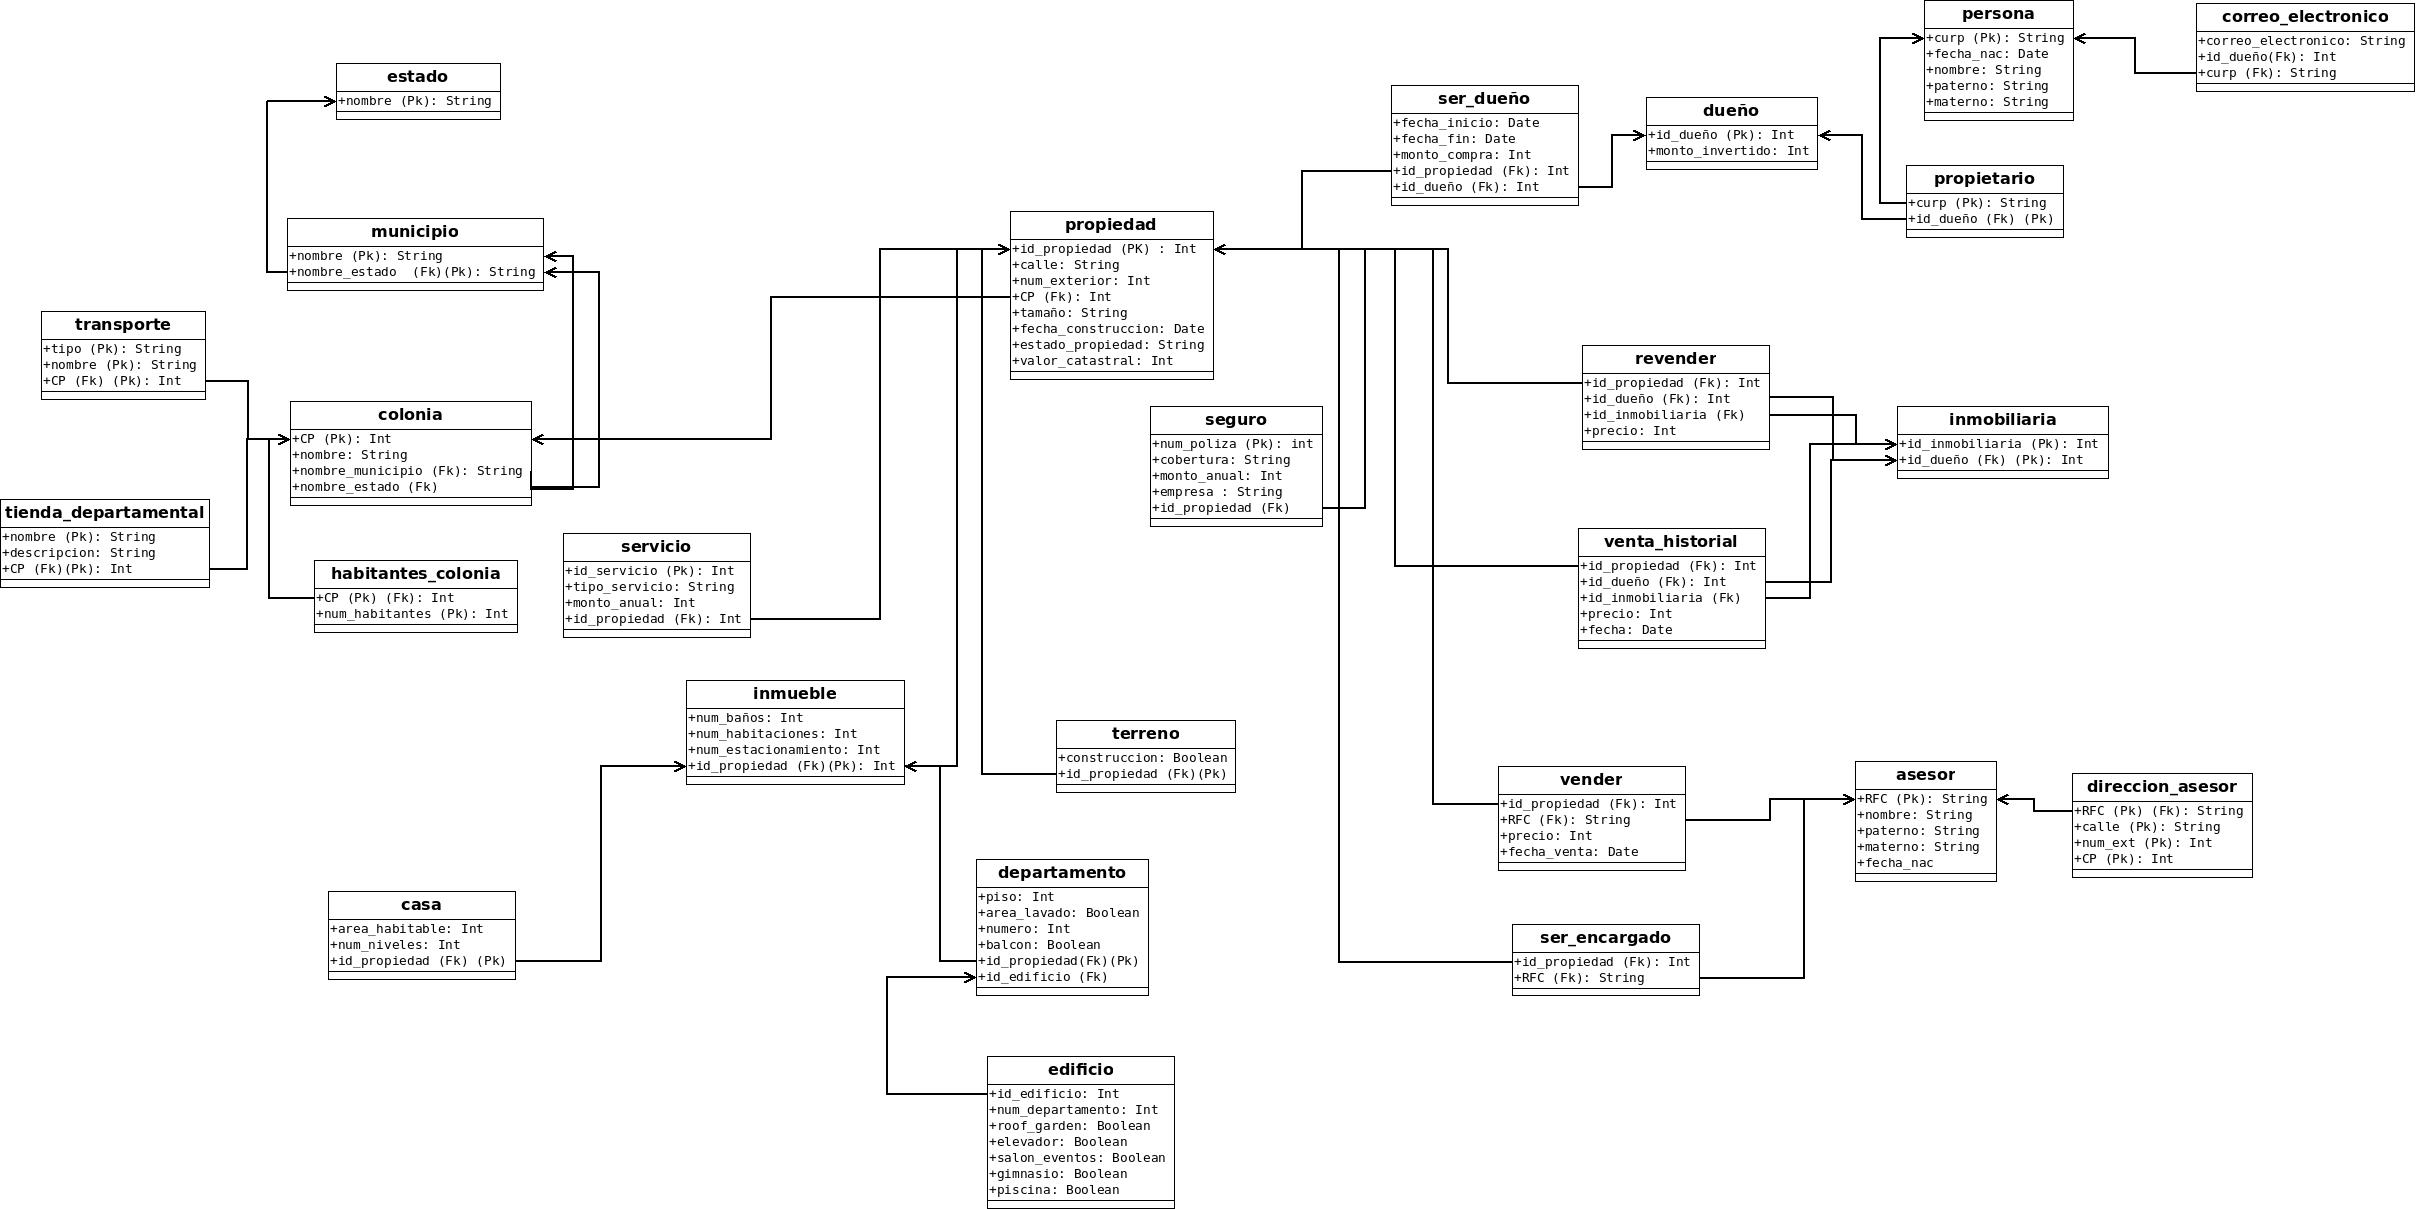
\includegraphics[width=1 \textwidth]{./modeloNormalizadoF.jpeg}
    		\caption{Esquema que corresponde a la normalización del esquema de la figura \ref{MR} usando normalización de BCNF.}
    	\end{figure}
    \end{center}
    
    
Finalmente, con el resultado de la normalización se crea  la base de datos usando el manejador de base de datos de Oracle, version 18.  \\  


    
\end{document}	
	
	
	
	
	
	
	
	